\documentclass[12pt,]{article}
\usepackage{lmodern}
\usepackage{amssymb,amsmath}
\usepackage{ifxetex,ifluatex}
\usepackage{fixltx2e} % provides \textsubscript
\ifnum 0\ifxetex 1\fi\ifluatex 1\fi=0 % if pdftex
  \usepackage[T1]{fontenc}
  \usepackage[utf8]{inputenc}
\else % if luatex or xelatex
  \ifxetex
    \usepackage{mathspec}
  \else
    \usepackage{fontspec}
  \fi
  \defaultfontfeatures{Ligatures=TeX,Scale=MatchLowercase}
\fi
% use upquote if available, for straight quotes in verbatim environments
\IfFileExists{upquote.sty}{\usepackage{upquote}}{}
% use microtype if available
\IfFileExists{microtype.sty}{%
\usepackage{microtype}
\UseMicrotypeSet[protrusion]{basicmath} % disable protrusion for tt fonts
}{}
\usepackage[margin=1in]{geometry}
\usepackage{hyperref}
\hypersetup{unicode=true,
            pdftitle={My first paper},
            pdfborder={0 0 0},
            breaklinks=true}
\urlstyle{same}  % don't use monospace font for urls
\usepackage{color}
\usepackage{fancyvrb}
\newcommand{\VerbBar}{|}
\newcommand{\VERB}{\Verb[commandchars=\\\{\}]}
\DefineVerbatimEnvironment{Highlighting}{Verbatim}{commandchars=\\\{\}}
% Add ',fontsize=\small' for more characters per line
\usepackage{framed}
\definecolor{shadecolor}{RGB}{248,248,248}
\newenvironment{Shaded}{\begin{snugshade}}{\end{snugshade}}
\newcommand{\KeywordTok}[1]{\textcolor[rgb]{0.13,0.29,0.53}{\textbf{#1}}}
\newcommand{\DataTypeTok}[1]{\textcolor[rgb]{0.13,0.29,0.53}{#1}}
\newcommand{\DecValTok}[1]{\textcolor[rgb]{0.00,0.00,0.81}{#1}}
\newcommand{\BaseNTok}[1]{\textcolor[rgb]{0.00,0.00,0.81}{#1}}
\newcommand{\FloatTok}[1]{\textcolor[rgb]{0.00,0.00,0.81}{#1}}
\newcommand{\ConstantTok}[1]{\textcolor[rgb]{0.00,0.00,0.00}{#1}}
\newcommand{\CharTok}[1]{\textcolor[rgb]{0.31,0.60,0.02}{#1}}
\newcommand{\SpecialCharTok}[1]{\textcolor[rgb]{0.00,0.00,0.00}{#1}}
\newcommand{\StringTok}[1]{\textcolor[rgb]{0.31,0.60,0.02}{#1}}
\newcommand{\VerbatimStringTok}[1]{\textcolor[rgb]{0.31,0.60,0.02}{#1}}
\newcommand{\SpecialStringTok}[1]{\textcolor[rgb]{0.31,0.60,0.02}{#1}}
\newcommand{\ImportTok}[1]{#1}
\newcommand{\CommentTok}[1]{\textcolor[rgb]{0.56,0.35,0.01}{\textit{#1}}}
\newcommand{\DocumentationTok}[1]{\textcolor[rgb]{0.56,0.35,0.01}{\textbf{\textit{#1}}}}
\newcommand{\AnnotationTok}[1]{\textcolor[rgb]{0.56,0.35,0.01}{\textbf{\textit{#1}}}}
\newcommand{\CommentVarTok}[1]{\textcolor[rgb]{0.56,0.35,0.01}{\textbf{\textit{#1}}}}
\newcommand{\OtherTok}[1]{\textcolor[rgb]{0.56,0.35,0.01}{#1}}
\newcommand{\FunctionTok}[1]{\textcolor[rgb]{0.00,0.00,0.00}{#1}}
\newcommand{\VariableTok}[1]{\textcolor[rgb]{0.00,0.00,0.00}{#1}}
\newcommand{\ControlFlowTok}[1]{\textcolor[rgb]{0.13,0.29,0.53}{\textbf{#1}}}
\newcommand{\OperatorTok}[1]{\textcolor[rgb]{0.81,0.36,0.00}{\textbf{#1}}}
\newcommand{\BuiltInTok}[1]{#1}
\newcommand{\ExtensionTok}[1]{#1}
\newcommand{\PreprocessorTok}[1]{\textcolor[rgb]{0.56,0.35,0.01}{\textit{#1}}}
\newcommand{\AttributeTok}[1]{\textcolor[rgb]{0.77,0.63,0.00}{#1}}
\newcommand{\RegionMarkerTok}[1]{#1}
\newcommand{\InformationTok}[1]{\textcolor[rgb]{0.56,0.35,0.01}{\textbf{\textit{#1}}}}
\newcommand{\WarningTok}[1]{\textcolor[rgb]{0.56,0.35,0.01}{\textbf{\textit{#1}}}}
\newcommand{\AlertTok}[1]{\textcolor[rgb]{0.94,0.16,0.16}{#1}}
\newcommand{\ErrorTok}[1]{\textcolor[rgb]{0.64,0.00,0.00}{\textbf{#1}}}
\newcommand{\NormalTok}[1]{#1}
\usepackage{longtable,booktabs}
\usepackage{graphicx,grffile}
\makeatletter
\def\maxwidth{\ifdim\Gin@nat@width>\linewidth\linewidth\else\Gin@nat@width\fi}
\def\maxheight{\ifdim\Gin@nat@height>\textheight\textheight\else\Gin@nat@height\fi}
\makeatother
% Scale images if necessary, so that they will not overflow the page
% margins by default, and it is still possible to overwrite the defaults
% using explicit options in \includegraphics[width, height, ...]{}
\setkeys{Gin}{width=\maxwidth,height=\maxheight,keepaspectratio}
\IfFileExists{parskip.sty}{%
\usepackage{parskip}
}{% else
\setlength{\parindent}{0pt}
\setlength{\parskip}{6pt plus 2pt minus 1pt}
}
\setlength{\emergencystretch}{3em}  % prevent overfull lines
\providecommand{\tightlist}{%
  \setlength{\itemsep}{0pt}\setlength{\parskip}{0pt}}
\setcounter{secnumdepth}{5}
% Redefines (sub)paragraphs to behave more like sections
\ifx\paragraph\undefined\else
\let\oldparagraph\paragraph
\renewcommand{\paragraph}[1]{\oldparagraph{#1}\mbox{}}
\fi
\ifx\subparagraph\undefined\else
\let\oldsubparagraph\subparagraph
\renewcommand{\subparagraph}[1]{\oldsubparagraph{#1}\mbox{}}
\fi

%%% Use protect on footnotes to avoid problems with footnotes in titles
\let\rmarkdownfootnote\footnote%
\def\footnote{\protect\rmarkdownfootnote}

%%% Change title format to be more compact
\usepackage{titling}

% Create subtitle command for use in maketitle
\newcommand{\subtitle}[1]{
  \posttitle{
    \begin{center}\large#1\end{center}
    }
}

\setlength{\droptitle}{-2em}

  \title{My first paper}
    \pretitle{\vspace{\droptitle}\centering\huge}
  \posttitle{\par}
    \author{Anna Quaglieri\footnote{Corresponding author:
  \href{mailto:anna.quaglieri16@gmail.com}{\nolinkurl{anna.quaglieri16@gmail.com}}}
\(^{1,2}\), Soroor Zadeh \(^{1,2}\)\\
\(^1\)Walter and Eliza Hall Institute, \(^2\)University of Melbourne}
    \preauthor{\centering\large\emph}
  \postauthor{\par}
    \date{}
    \predate{}\postdate{}
  
\usepackage{booktabs}
\usepackage{longtable}
\usepackage{array}
\usepackage{multirow}
\usepackage{wrapfig}
\usepackage{float}
\usepackage{colortbl}
\usepackage{pdflscape}
\usepackage{tabu}
\usepackage{threeparttable}
\usepackage{threeparttablex}
\usepackage[normalem]{ulem}
\usepackage{makecell}
\usepackage{xcolor}

\usepackage{float} \floatplacement{figure}{H} \newcommand{\beginsupplement}{\setcounter{table}{0}  \renewcommand{\thetable}{S\arabic{table}} \setcounter{figure}{0} \renewcommand{\thefigure}{S\arabic{figure}}} \usepackage{setspace}\doublespacing \usepackage{lineno} \linenumbers

\begin{document}
\maketitle
\begin{abstract}
Hopefully with this minimal example you will appreciate the robustness
and flexibility of \texttt{bookdown} and you will start writing amazing
reproducible documents!!
\end{abstract}

{
\setcounter{tocdepth}{2}
\tableofcontents
}
\newpage

\section{Introduction}\label{introduction}

\label{sec:intro}

This is my introduction to the flexible \texttt{bookdown} (Xie
\protect\hyperlink{ref-bookdown}{2016}) package.

\texttt{bookdown} extends the syntax provided by R Markdown, allowing
automatic numbering of figures / tables / equations, and
cross-references within a single documents.

\section{Results}\label{results}

\label{sec:res}

All the Figures created by the chunks in this article will be saved into
the \texttt{img/} which is created in the setup chunk at the beginning
of this document.

\begin{Shaded}
\begin{Highlighting}[]
\NormalTok{knitr}\OperatorTok{::}\NormalTok{opts_chunk}\OperatorTok{$}\KeywordTok{set}\NormalTok{(}\DataTypeTok{echo =} \OtherTok{TRUE}\NormalTok{,}\DataTypeTok{fig.height =} \DecValTok{5}\NormalTok{,}\DataTypeTok{fig.width =} \DecValTok{5}\NormalTok{,}\DataTypeTok{fig.path =} \StringTok{"img/"}\NormalTok{,}\DataTypeTok{tidy =} \OtherTok{TRUE}\NormalTok{)}
\end{Highlighting}
\end{Shaded}

\subsection{\texorpdfstring{Some \texttt{LaTex}
options!}{Some LaTex options!}}\label{some-latex-options}

\begin{itemize}
\tightlist
\item
  Try removing the following from the \texttt{YAML}!
\end{itemize}

\begin{Shaded}
\begin{Highlighting}[]
\OtherTok{---}
\NormalTok{\textbackslash{}usepackage}\KeywordTok{\{}\NormalTok{setspace}\KeywordTok{\}}\NormalTok{\textbackslash{}doublespacing}
\NormalTok{\textbackslash{}usepackage}\KeywordTok{\{}\NormalTok{lineno}\KeywordTok{\}}
\NormalTok{\textbackslash{}linenumbers}
\OtherTok{---}
\end{Highlighting}
\end{Shaded}

\begin{itemize}
\tightlist
\item
  Try adding the LaTex command
  \texttt{\textbackslash{}usepackage\{endfloat\}} after
  \texttt{header-includes:} in the \texttt{YAML}
\end{itemize}

\subsection{Generate figures within a
chunk}\label{generate-figures-within-a-chunk}

\begin{Shaded}
\begin{Highlighting}[]
\KeywordTok{plot}\NormalTok{(}\KeywordTok{density}\NormalTok{(}\KeywordTok{rnorm}\NormalTok{(}\DecValTok{100}\NormalTok{)))}
\end{Highlighting}
\end{Shaded}

\begin{figure}
\centering
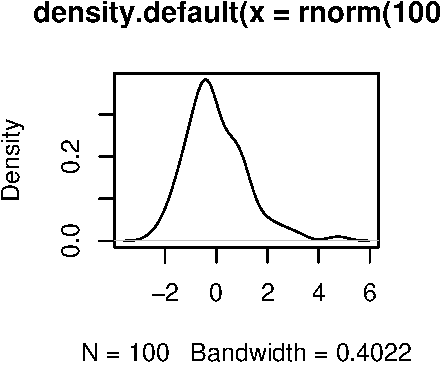
\includegraphics{img/bell-curve-1.pdf}
\caption{\label{fig:bell-curve}Red trees in autumn}
\end{figure}

It's a pretty cool bell curve in Figure \ref{fig:bell-curve}.

\begin{itemize}
\tightlist
\item
  Don't use \texttt{\_} in labels! This is taken from \texttt{bookdown}
  book: \emph{If you want to cross-reference figures or tables generated
  from a code chunk, please make sure the chunk label only contains
  alphanumeric characters (a-z, A-Z, 0-9), slashes (/), or dashes (-).}
\end{itemize}

\subsection{\texorpdfstring{Insert \texttt{png}
figures}{Insert png figures}}\label{insert-png-figures}

\begin{Shaded}
\begin{Highlighting}[]
\NormalTok{img <-}\StringTok{ }\NormalTok{png}\OperatorTok{::}\KeywordTok{readPNG}\NormalTok{(}\StringTok{"img/kooka.png"}\NormalTok{)}
\KeywordTok{grid.raster}\NormalTok{(img)}
\end{Highlighting}
\end{Shaded}

\begin{figure}
\centering
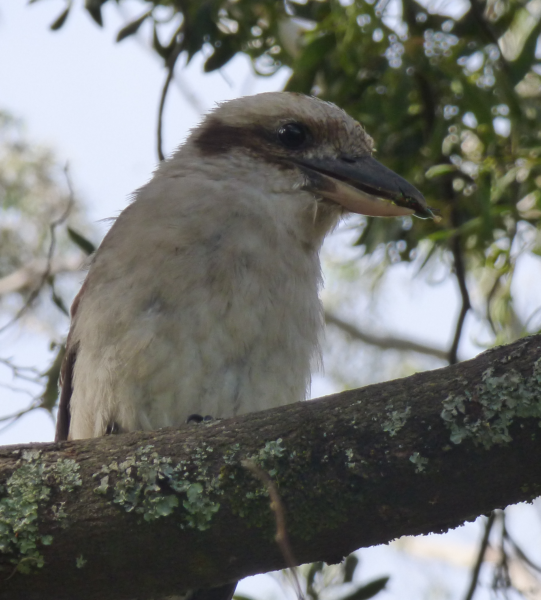
\includegraphics{img/loud-kooka-1.pdf}
\caption{\label{fig:loud-kooka}Loud Kookabara}
\end{figure}

\subsection{\texorpdfstring{Insert \texttt{pdf} figures with
\texttt{knitr::include\_graphics}}{Insert pdf figures with knitr::include\_graphics}}\label{insert-pdf-figures-with-knitrinclude_graphics}

\begin{Shaded}
\begin{Highlighting}[]
\NormalTok{knitr}\OperatorTok{::}\KeywordTok{include_graphics}\NormalTok{(}\StringTok{"img/reproducible-documents.pdf"}\NormalTok{)}
\end{Highlighting}
\end{Shaded}

\begin{figure}
\centering
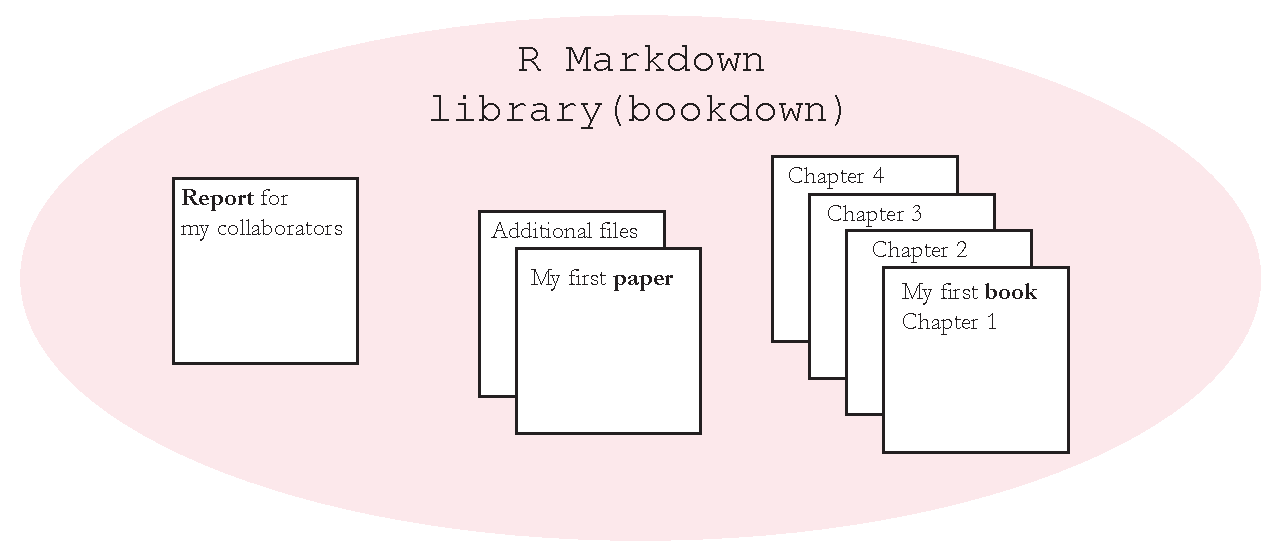
\includegraphics{img/reproducible-documents.pdf}
\caption{\label{fig:bookdown-docs}All types of documents with
\texttt{bookdown}}
\end{figure}

\subsection{\texorpdfstring{Insert tables with
\texttt{knitr::kable}}{Insert tables with knitr::kable}}\label{insert-tables-with-knitrkable}

\begin{Shaded}
\begin{Highlighting}[]
\NormalTok{tab <-}\StringTok{ }\NormalTok{knitr}\OperatorTok{::}\KeywordTok{kable}\NormalTok{(}\KeywordTok{head}\NormalTok{(diamonds), }\DataTypeTok{caption =} \StringTok{"A table of the first 10 rows and three columns of the diamonds data."}\NormalTok{, }
    \DataTypeTok{booktabs =} \OtherTok{TRUE}\NormalTok{)}

\NormalTok{kableExtra}\OperatorTok{::}\KeywordTok{kable_styling}\NormalTok{(tab, }\DataTypeTok{latex_options =} \StringTok{"hold_position"}\NormalTok{)}
\end{Highlighting}
\end{Shaded}

\begin{table}[!h]

\caption{\label{tab:tree-diamonds}A table of the first 10 rows and three columns of the diamonds data.}
\centering
\begin{tabular}{rlllrrrrrr}
\toprule
carat & cut & color & clarity & depth & table & price & x & y & z\\
\midrule
0.23 & Ideal & E & SI2 & 61.5 & 55 & 326 & 3.95 & 3.98 & 2.43\\
0.21 & Premium & E & SI1 & 59.8 & 61 & 326 & 3.89 & 3.84 & 2.31\\
0.23 & Good & E & VS1 & 56.9 & 65 & 327 & 4.05 & 4.07 & 2.31\\
0.29 & Premium & I & VS2 & 62.4 & 58 & 334 & 4.20 & 4.23 & 2.63\\
0.31 & Good & J & SI2 & 63.3 & 58 & 335 & 4.34 & 4.35 & 2.75\\
\addlinespace
0.24 & Very Good & J & VVS2 & 62.8 & 57 & 336 & 3.94 & 3.96 & 2.48\\
\bottomrule
\end{tabular}
\end{table}

We created the simple Table \ref{tab:tree-diamonds}. See more on tables
and long tables \url{https://bookdown.org/yihui/bookdown/tables.html}.

\subsection{\texorpdfstring{Extra tips: Setup your bibliography with
\texttt{utils::citation}}{Extra tips: Setup your bibliography with utils::citation}}\label{extra-tips-setup-your-bibliography-with-utilscitation}

\begin{Shaded}
\begin{Highlighting}[]
\KeywordTok{print}\NormalTok{(utils}\OperatorTok{::}\KeywordTok{citation}\NormalTok{(}\StringTok{"rticles"}\NormalTok{), }\DataTypeTok{bibtex =} \OtherTok{TRUE}\NormalTok{)}
\end{Highlighting}
\end{Shaded}

\begin{verbatim}
## 
## To cite package 'rticles' in publications use:
## 
##   JJ Allaire, Yihui Xie, R Foundation, Hadley Wickham, Journal of
##   Statistical Software, Ramnath Vaidyanathan, Association for
##   Computing Machinery, Carl Boettiger, Elsevier, Karl Broman,
##   Kirill Mueller, Bastiaan Quast, Randall Pruim, Ben Marwick,
##   Charlotte Wickham, Oliver Keyes, Miao Yu, Daniel Emaasit,
##   Thierry Onkelinx, Alessandro Gasparini, Marc-Andre Desautels,
##   Dominik Leutnant, MDPI, Oğuzhan Öğreden, Dalton Hance and Daniel
##   Nüst (2018). rticles: Article Formats for R Markdown. R package
##   version 0.6. https://CRAN.R-project.org/package=rticles
## 
## A BibTeX entry for LaTeX users is
## 
##   @Manual{,
##     title = {rticles: Article Formats for R Markdown},
##     author = {JJ Allaire and Yihui Xie and {R Foundation} and Hadley Wickham and {Journal of Statistical Software} and Ramnath  Vaidyanathan and {Association for Computing Machinery} and Carl Boettiger and {Elsevier} and Karl Broman and Kirill Mueller and Bastiaan Quast and Randall  Pruim and Ben Marwick and Charlotte Wickham and Oliver Keyes and Miao Yu and Daniel Emaasit and Thierry Onkelinx and Alessandro Gasparini and Marc-Andre Desautels and Dominik Leutnant and {MDPI} and Oğuzhan Öğreden and Dalton Hance and Daniel Nüst},
##     year = {2018},
##     note = {R package version 0.6},
##     url = {https://CRAN.R-project.org/package=rticles},
##   }
\end{verbatim}

\subsection{Reference/Re-number files in supplementary
material}\label{referencere-number-files-in-supplementary-material}

Have a look at the beautiful autumn trees in Figure \ref{fig:red-trees}.

\subsection{Collaboration with
co-authors}\label{collaboration-with-co-authors}

\begin{itemize}
\tightlist
\item
  Setup a \texttt{GitHub} account and push/pull changes with your
  collaborators
\item
  Checkout \href{https://www.overleaf.com/}{Overleaf} for real-time
  collaboration on LaTex file. Have a read at this
  \href{https://medium.com/@arinbasu/a-tutorial-on-how-to-interface-an-r-notebook-with-overleaf-11f23c306cfd}{blog
  post} that discuss working with Git, RStudio and Overleaf at the same
  time. The drawback is that, while it is easy to go from \texttt{Rmd}
  to \texttt{.tex} with the \texttt{YAML} option
  \texttt{keep\_tex:\ true}, it is not the same on the other way around.
  However, it is worth checking it out since it offers plenty of journal
  LaTex templates!
\end{itemize}

\section{Conclusions}\label{conclusions}

Hopefully now you have a pretty good overview of the options offered by
\texttt{bookdown}! Also, the best way to learn is to go through other
people's GitHub accounts and have a look at how they do things as well
as ask questions!

\newpage

\section*{Supplementary Material}\label{supplementary-material}
\addcontentsline{toc}{section}{Supplementary Material}

\beginsupplement

\subsection*{A beautiful autumn tree}\label{a-beautiful-autumn-tree}
\addcontentsline{toc}{subsection}{A beautiful autumn tree}

\begin{Shaded}
\begin{Highlighting}[]
\NormalTok{img <-}\StringTok{ }\NormalTok{png}\OperatorTok{::}\KeywordTok{readPNG}\NormalTok{(}\StringTok{"img/trees.png"}\NormalTok{)}
\NormalTok{grid}\OperatorTok{::}\KeywordTok{grid.raster}\NormalTok{(img)}
\end{Highlighting}
\end{Shaded}

\begin{figure}
\centering
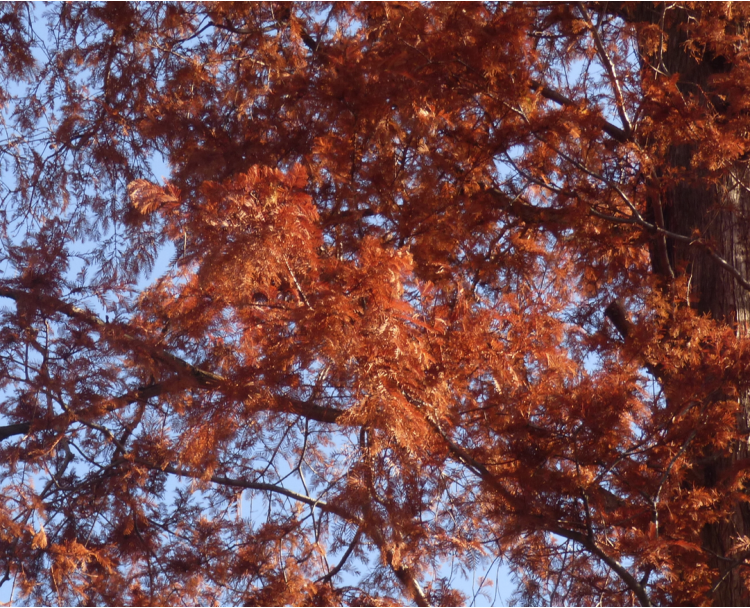
\includegraphics{img/red-trees-1.pdf}
\caption{\label{fig:red-trees}Autumn trees at the University of Melbourne}
\end{figure}

\newpage

\section*{References}\label{references}
\addcontentsline{toc}{section}{References}

\subsection{Interesting blogposts}\label{interesting-blogposts}

\begin{itemize}
\item
  \emph{Interface R with Overleaf}
  \url{https://medium.com/@arinbasu/a-tutorial-on-how-to-interface-an-r-notebook-with-overleaf-11f23c306cfd}
\item
  Minimal \texttt{bookdown} template for scientific papers
  \url{http://landscapeportal.org/blog/2017/09/06/r-markdown-template-for-a-scientific-manuscript/}
\item
  \href{https://github.com/earowang/paper-calendar-vis}{Earo Wang papers
  on GitHub} and helpful suggestions via email!
\end{itemize}

\hypertarget{refs}{}
\hypertarget{ref-bookdown}{}
Xie, Yihui. 2016. \emph{Bookdown: Authoring Books and Technical
Documents with R Markdown}. Boca Raton, Florida: Chapman; Hall/CRC.
\url{https://github.com/rstudio/bookdown}.


\end{document}
